\documentclass[slidestop]{beamer}

\usepackage[english]{babel}
\usepackage{graphicx}
\usepackage{hyperref}

\title{Open and Reproducible Scientific Programming}
\providecommand{\myConference}{Lab-J work discussion}
\providecommand{\myDate}{Wednesday, 30 Januari 2013}
\author{Martijn Vermaat}
\providecommand{\myGroup}{}
\providecommand{\myDepartment}{Department of Human Genetics}
\providecommand{\myCenter}{Center for Human and Clinical Genetics}
\providecommand{\lastCenterLogo}{
  \raisebox{-0.1cm}{
    
\includegraphics[height = 1cm]{lgtc_logo}
  }
}
\providecommand{\lastRightLogo}{
  
\includegraphics[height = 0.7cm]{nbic_logo}
  %\includegraphics[height = 0.8cm]{nwo_logo_en}
}

\usetheme{lumc}

\begin{document}

% This disables the \pause command, handy in the editing phase.
%\renewcommand{\pause}{}

% Make the title page.
\bodytemplate

%\section{Introduction}

\frame{
  \frametitle{Open and Reproducible Scientific Programming}
  \tableofcontents
}

\section{Academic publishing}

\begin{frame}
  \frametitle{Scientific findings}
  Should be
  \begin{itemize}
    \item Replicable

      \uncover<2->{Verify method and result}
    \item Reproducible

      \uncover<3->{Verify result by other means}
    \item Reusable

      \uncover<4->{Build on previous results}
  \end{itemize}
\end{frame}

\begin{frame}
  \frametitle{Data}
  \begin{itemize}[<+->]
    \item Data should be published with the paper
    \item Policies often include additional requirements
    \item Data standards
    \item Specific databases
    \item E.g. publish genomic variants
  \end{itemize}
\end{frame}

\begin{frame}
  \frametitle{Data policy example}
  \begin{quote}
    Authors must follow standards and practice for data deposition in
    publicly available resources including those created for gene sequences,
    microarray expression, structural studies, and similar kinds of
    data. Failure to comply with community standards may result in rejection.
  \end{quote}
  (PLOS ONE Publication Criteria)
\end{frame}

\begin{frame}
  \frametitle{Source code}
  \begin{itemize}[<+->]
    \item Results often depend on computational analysis
    \item Source code should be published with the paper
    \item Are there policies?
  \end{itemize}
\end{frame}

\begin{frame}
  \frametitle{Source code policy example (1)}
  \begin{quote}
    Of the 20 most-cited journals in 2010 from all fields of science, only
    three (including Science) have editorial policies requiring
    availability of computer source code upon publication. This stands in stark
    contrast to near-universal agreement among the 20 on policies regarding
    availability of data and other enabling materials.
  \end{quote}
  (A. Morin et al. Shining Light into Black Boxes. Science 13 April 2012:
  Vol. 336 no. 6078 pp. 159--160)
\end{frame}

\begin{frame}
  \frametitle{Source code policy example (2)}
  \begin{quote}
    Although it is now accepted that data should be made available on
    request, the current regulations regarding the availability of software
    are inconsistent. We argue that, with some exceptions, anything less than
    the release of source programs is intolerable for results that depend on
    computation.
  \end{quote}
  (D.C. Ince et al. The case for open computer programs. Nature 482, 485--488
  (23 February 2012))
\end{frame}

\begin{frame}
  \frametitle{Source code policy example (3)}
  \begin{quote}
    Nature does not require authors to make code available, but we do
    expect a description detailed enough to allow others to write their
    own code to do a similar analysis.
  \end{quote}
  (Devil in the details. Nature 470, 305--306 (17 February 2011))
\end{frame}

\begin{frame}
  \frametitle{Source code policy example (4)}
  \begin{quote}
    The editors of Bioinformatics encourage authors to make their source
    code available and, if possible, to provide access through an open source
    license (see http://www.opensource.org for examples). Authors should make
    every effort to use URLs that will remain stable. At the minimum, authors
    must provide one of: webserver, source code or binary.
  \end{quote}
  (Bioinformatics Instructions to Authors)
\end{frame}

\begin{frame}
  \frametitle{Source code policy example (5)}
  \begin{quote}
    To address the growing complexity of data and analyses, Science is
    extending our data access requirement listed above to include computer
    codes involved in the creation or analysis of data.
  \end{quote}
  (B. Hanson et al. Making Data Maximally Available. Science 11 February 2011:
  Vol. 331 no. 6018 p. 649)
\end{frame}

% Todo: new section?

\begin{frame}
  \frametitle{Value of software}
  \begin{quote}
    Time spent on software development that doesn't result in
    widely-recognized deliverables such as publications or grants is essentially
    time wasted, and will be inversely correlated with your chances of success
    as an academic.
  \end{quote}
  \vspace{1cm}
  \pause
  \begin{itemize}[<+->]
    \item What counts in academia?
    \item Reputation
    \item Recognize software as a product of research
  \end{itemize}
\end{frame}

\begin{frame}
  \frametitle{Value of software}
  Recent change to the NSF grant proposal guide:
  \begin{quote}
    The acknowledgement of datasets, patents, software, and copyrights as
    citable products of research, eligible for inclusion in a researcher's
    biosketch.
  \end{quote}
  (National Science Foundation, January 2013)
\end{frame}

\begin{frame}
  \frametitle{Example: 1000 Genomes Project}
  \begin{quote}
    The 1000 Genomes Project, for example, a project to sequence and
    analyse more than a thousand genomes, has carefully detailed its
    workflows, and makes both its data and its procedures available for
    the world to see.
  \end{quote}
  (Devil in the details. Nature 470, 305--306 (17 February 2011))
\end{frame}

\begin{frame}
  \frametitle{Example: ENCODE}
  \begin{quote}
    As part of the supplementary material for this paper, we have established
    a virtual machine instance of the software, using the code bundles from
    ftp.ebi.ac.uk/pub/databases/ensembl/encode/supplementary/, where each
    analysis program has been tested and run.
  \end{quote}
  \begin{quote}
    Where possible the VM enables complete reproduction of the analysis as it
    was performed to generate the figures, tables or other information.
  \end{quote}
  (ENCODE Virtual Machine and Cloud Resource)
\end{frame}

\section*{}

\frame{
  \frametitle{Open and Reproducible Scientific Programming}
  \tableofcontents
}

\section{Reasons not to open your source code}

\begin{frame}
  \frametitle{1. ``Obligates me to support it''}
  \pause
  No, it doesn't.
\end{frame}

{
  \setbeamercolor{background canvas}{bg=}
  \usebackgroundtemplate{
    \parbox[c][\paperheight]{\paperwidth}{%
      \vfill \begin{center}
      \includegraphics[clip=true,trim=0cm 17cm 0cm 0cm,width=\paperwidth,keepaspectratio=true]{publish}
      \end{center} \vfill}
  }
  \frame{}
}

\begin{frame}
  \frametitle{2. ``I'm ashamed of my bad code''}
  \pause
  \begin{itemize}[<+->]
    \item If it is good enough to do the job, it's good enough to be released
      (in support of the publication)
    \item Opening might improve it
    \item CRAPL license:
      \begin{enumerate}
        \item Source and modifications used to validate scientific claims be
          released with those claims
        \item Authors are absolved of shame, embarrassment and ridicule for
          ugly code
      \end{enumerate}
  \end{itemize}
\end{frame}

\begin{frame}
  \frametitle{3. ``It takes time/effort/money''}
  \pause
  \begin{itemize}
    \item It doesn't have to
    \item For scientists, publication signifies perfectionism
    \item Very good infrastructure is available (GitHub, Bitbucket, Google
      Code, SourceForge)
    \item These are free and easy to use
  \end{itemize}
\end{frame}

\begin{frame}
  \frametitle{4. ``They will steal my idea''}
  \pause
  \begin{itemize}
    \item I think this rarely matters in practice
    \item If you must, await publication
    \item Getting it out claims territory %establishes precedence
  \end{itemize}
\end{frame}

{
  \setbeamercolor{background canvas}{bg=}
  \usebackgroundtemplate{
    \parbox[c][\paperheight]{\paperwidth}{%
      \vfill \begin{center}
      
\includegraphics[width=0.9\paperwidth,keepaspectratio=true]{preprints1}
      \end{center} \vfill}
  }
  \frame{}
}

{
  \setbeamercolor{background canvas}{bg=}
  \usebackgroundtemplate{
    \parbox[c][\paperheight]{\paperwidth}{%
      \vfill \begin{center}
      
\includegraphics[width=0.9\paperwidth,keepaspectratio=true]{preprints2}
      \end{center} \vfill}
  }
  \frame{}
}

\begin{frame}
  \frametitle{5. ``An algorithmic description is good enough''}
  \pause
  \begin{itemize}
    \item It really isn't
    \item Descriptions are ambiguous and imperfect
    \item Makes replication impossible
    \item Makes reuse impossible
  \end{itemize}
\end{frame}

\section*{}

\frame{
  \frametitle{Open and Reproducible Scientific Programming}
  \tableofcontents
}

\section{Sharing computational analyses}

\begin{frame}
  \frametitle{Replicability}
  Not only for verification, also to regenerate lost data and to generate
  further data.

  \vspace{0.5cm}
  \pause

  Requirements:
  \begin{enumerate}
    \item Same input data
    \item Same build tools and settings
    \item Same source code
    \item Same software settings
    \item Same OS and environment
    \item Same hardware
  \end{enumerate}

  \vspace{0.5cm}
  \pause

  Provenance needed
\end{frame}

\begin{frame}
  \frametitle{Data analysis}
  \begin{itemize}
    \item<1-> Many workflow systems exist
    \item<2-> myExperiment to share workflows
    \item<3-> Taverna (using web services)
    \item<4-> A more extreme approach:
  \end{itemize}

  \uncover<4->{
  \begin{quote}
    We propose capturing and exchanging computational pipelines using
    complete digital representations of the entire computing environment
    needed to execute the pipeline.
  \end{quote}
  (J.T. Dudley et al. In silico research in the era of cloud computing. Nature
  Biotechnology 28, 1181--1185 (2010))
  }
\end{frame}

\begin{frame}
  \frametitle{Integrate code with data, figures, and text}
  \begin{itemize}[<+->]
    \item Literate programming (e.g. Sweave)
    \item IPython Notebook
    \item Great for exploratory research
  \end{itemize}
\end{frame}

{
  \setbeamercolor{background canvas}{bg=}
  \usebackgroundtemplate{
    \parbox[c][\paperheight]{\paperwidth}{%
      \vfill \begin{center}
      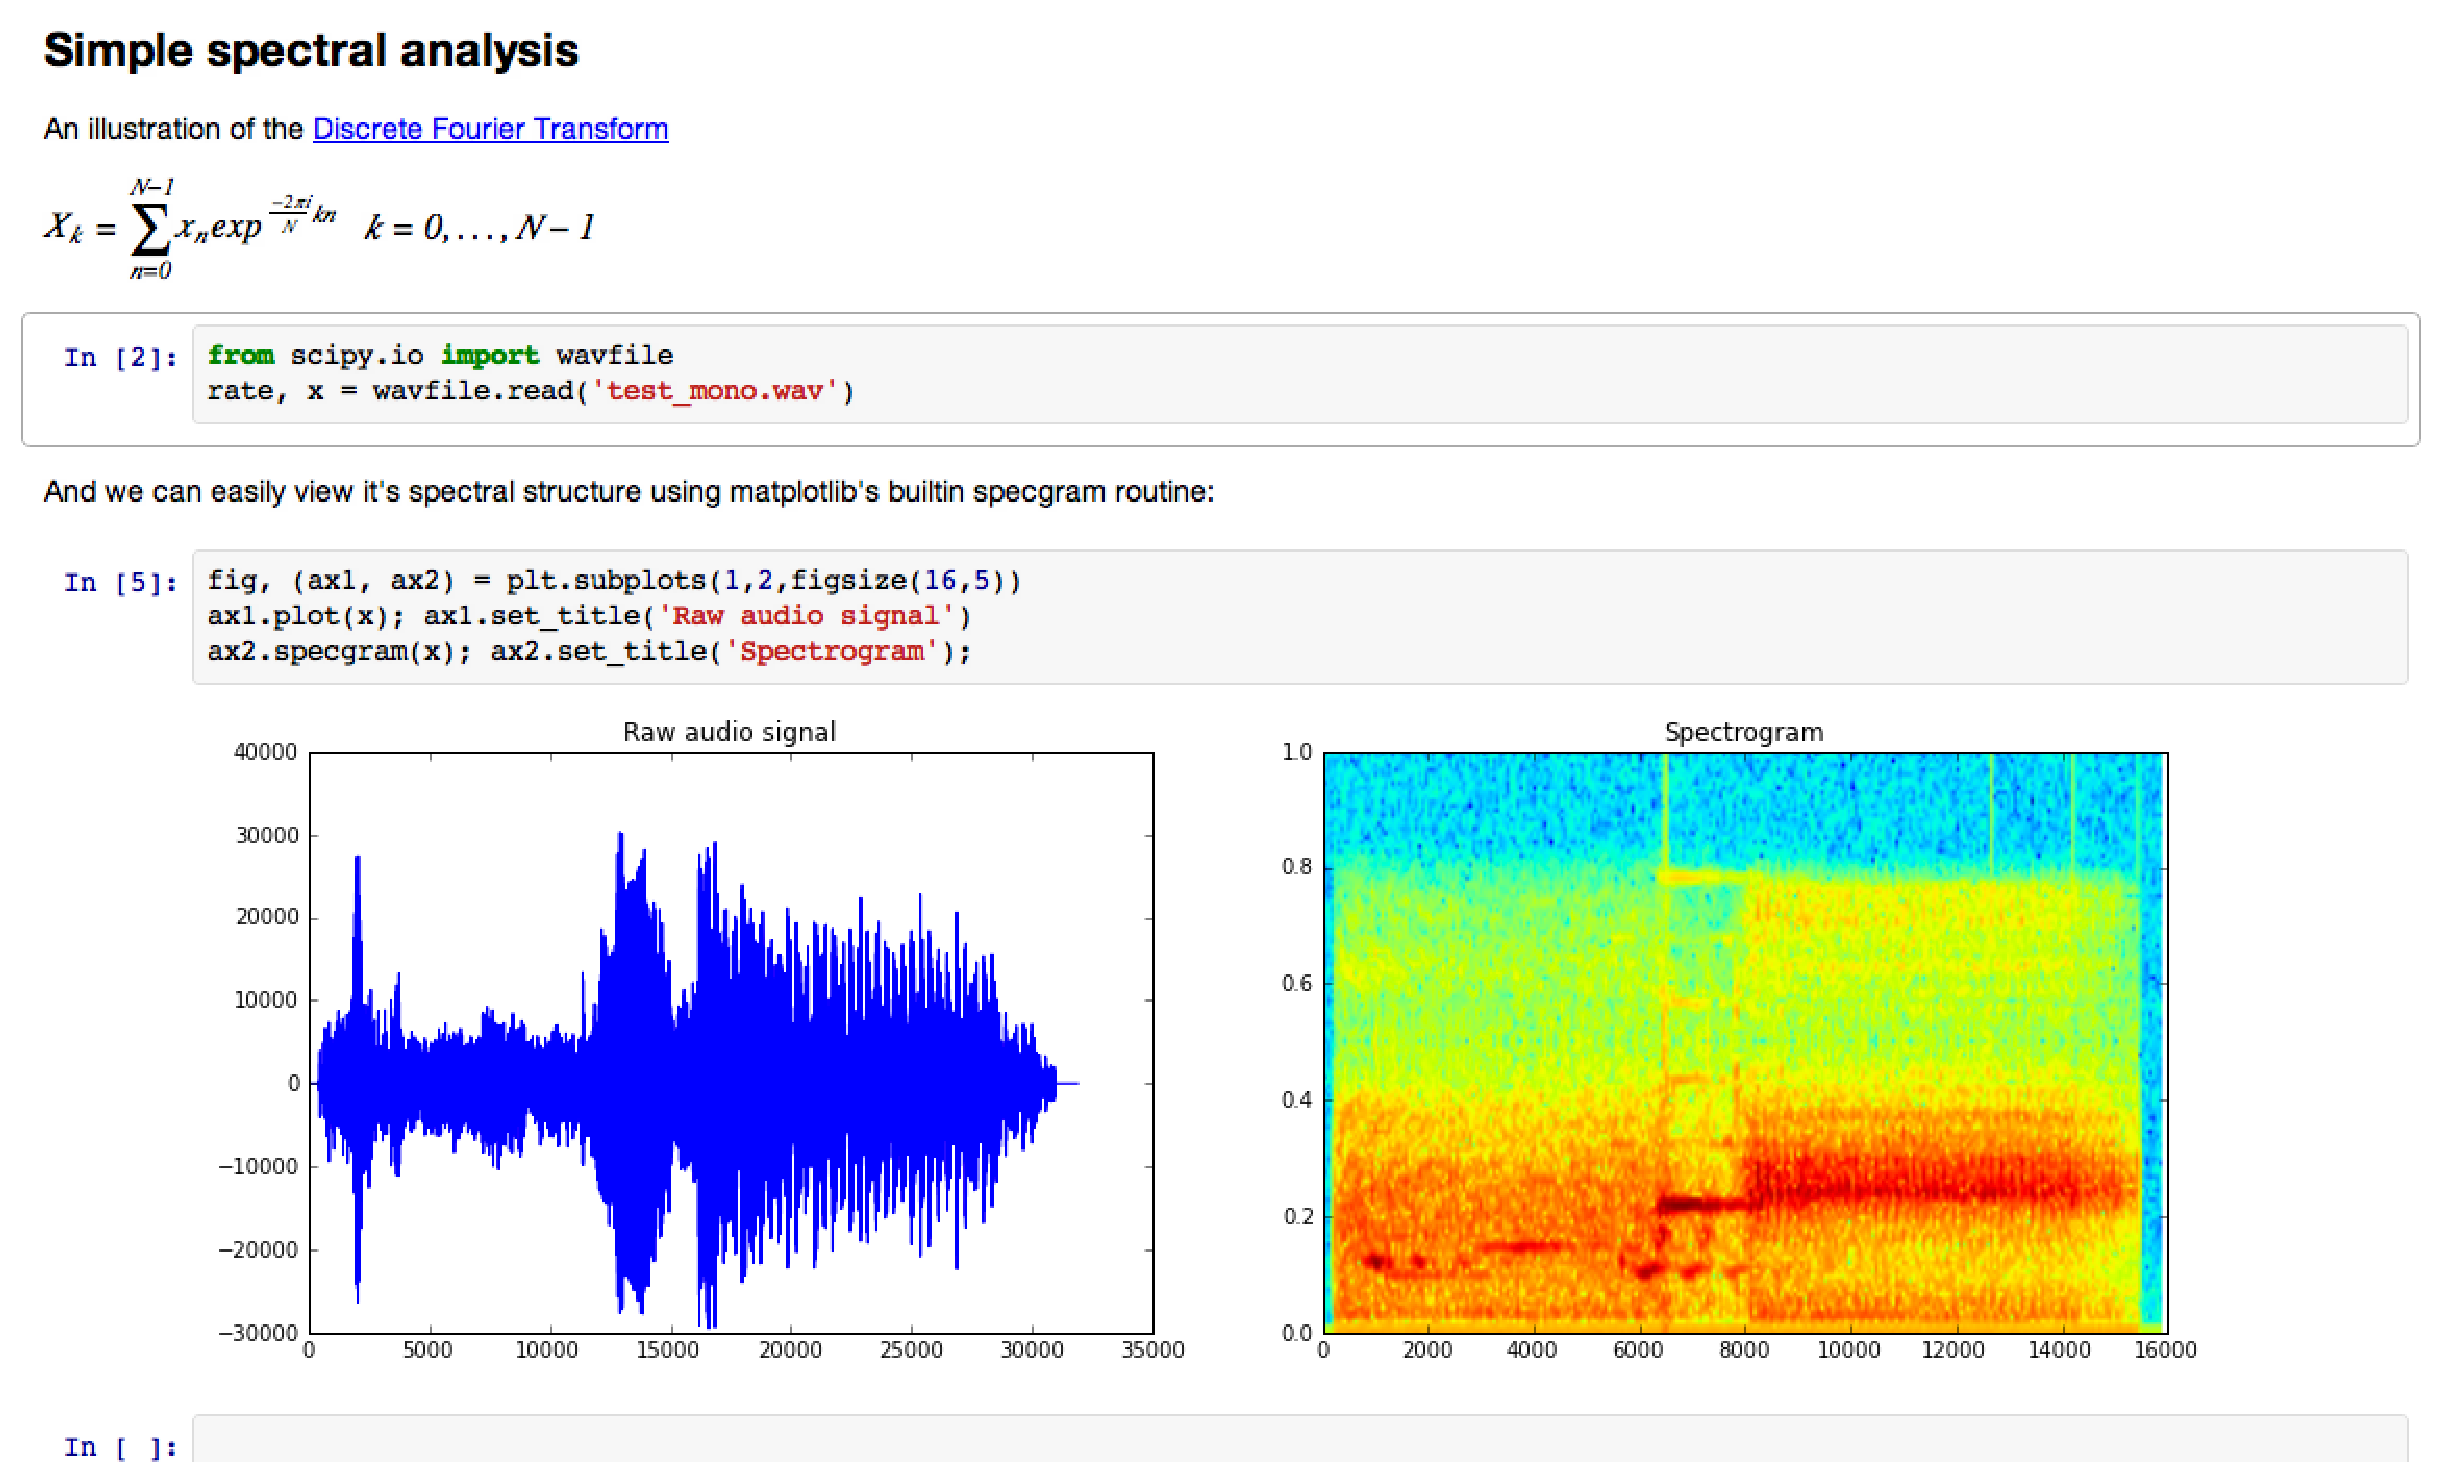
\includegraphics[width=0.9\paperwidth,keepaspectratio=true]{notebook}
      \end{center} \vfill}
  }
  \frame{}
}

\section*{}

\frame{
  \frametitle{Open and Reproducible Scientific Programming}
  \tableofcontents
}

\section{Best practices}

{
  \setbeamercolor{background canvas}{bg=}
  \usebackgroundtemplate{
    \parbox[c][\paperheight]{\paperwidth}{%
      \vfill \begin{center}
      
\includegraphics[width=0.55\paperwidth,keepaspectratio=true]{wtfm}
      \end{center} \vfill}
  }
  \frame{}
}

\begin{frame}
  \frametitle{The next step}
  \begin{itemize}
    \item We can do better than just having code
    \item Policies should define additional requirements
    \item Follow best practices (compare data standards)
    \item Academcis are not necessarily good programmers
  \end{itemize}
\end{frame}

{
  \setbeamercolor{background canvas}{bg=}
  \usebackgroundtemplate{
    \parbox[c][\paperheight]{\paperwidth}{%
      \vfill \begin{center}
      \includegraphics[clip=true,trim=1cm 10cm 3cm 0cm,width=\paperwidth,keepaspectratio=true]{compute}
      \end{center} \vfill}
  }
  \frame{}
}

\begin{frame}
  \frametitle{Rules, commandments, and best practices}
  Prli\'c A, Procter JB. {\bf Ten Simple Rules for the Open Development of
    Scientific Software}. PLoS Comput Biol 8(12), 2012.

  \vspace{0.5cm}

  Vince Buffalo. {\bf The ten commandments of scientific coding}. Published on
  GitHub, August 10, 2012.

  \vspace{0.5cm}

  Wilson et al. {\bf Best Practices for Scientific Computing}. Preprint,
  arXiv:1210.0530, 29 Nov 2012.
\end{frame}

\begin{frame}
  \frametitle{Ten simple rules for the open development of scientific
    software}
  \begin{enumerate}
    \item Don't Reinvent the Wheel
    \item Code Well
    \item Be Your Own User
    \item Be Transparent
    \item Be Simple
    \item Don't Be a Perfectionist
    \item Nurture and Grow Your Community
    \item Promote Your Project
    \item Find Sponsors
    \item Science Counts
  \end{enumerate}
\end{frame}

{
  \setbeamercolor{background canvas}{bg=}
  \usebackgroundtemplate{
    \parbox[c][\paperheight]{\paperwidth}{%
      \vfill \begin{center}
      
\includegraphics[width=0.9\paperwidth,keepaspectratio=true]{commandments}
      \end{center} \vfill}
  }
  \frame{}
}

\begin{frame}
  \frametitle{The ten commandments of scientific coding}
  \begin{enumerate}
    \item Thou shall use version control
    \item Thou shall comment thy code
    \item Thou shall use existing libraries whenever possible
    \item Thou shall try to unit test
    \item Thou shall not make up statistical procedures
    \item Thou shall read code other than thy own
    \item Thou shall write documentation
    \item Thou shall beware of floating point issues
    \item Thou shall write modular code
    \item Thou shall follow coding standards
  \end{enumerate}
\end{frame}

\begin{frame}
  \frametitle{The ten commandments of scientific coding}
  \begin{enumerate}
    \item {\bf Thou shall use version control}
    \item Thou shall comment thy code
    \item Thou shall use existing libraries whenever possible
    \item Thou shall try to unit test
    \item Thou shall not make up statistical procedures
    \item Thou shall read code other than thy own
    \item Thou shall write documentation
    \item Thou shall beware of floating point issues
    \item Thou shall write modular code
    \item Thou shall follow coding standards
  \end{enumerate}
\end{frame}

\begin{frame}
  \frametitle{Thou shall use version control}
  Two main uses:
  \pause
  \begin{enumerate}[<+->]
    \item Keeping track of files, versions, changes
    \item Collaboration
  \end{enumerate}

  \vspace{1cm}
  \pause

  Everything that has been created manually goes in.

  \vspace{1cm}
  \pause

  Being able to go back to computation of previous results aids
  replicability.
\end{frame}

\begin{frame}
  \frametitle{The ten commandments of scientific coding}
  \begin{enumerate}
    \item Thou shall use version control
    \item Thou shall comment thy code
    \item {\bf Thou shall use existing libraries whenever possible}
    \item Thou shall try to unit test
    \item Thou shall not make up statistical procedures
    \item Thou shall read code other than thy own
    \item Thou shall write documentation
    \item Thou shall beware of floating point issues
    \item Thou shall write modular code
    \item Thou shall follow coding standards
  \end{enumerate}
\end{frame}

\begin{frame}
  \frametitle{Thou shall use existing libraries whenever possible}
  \begin{itemize}[<+->]
    \item Re-use instead of rewrite
    \item Search on Google, GitHub, etc
    \item Document dependencies and their versions
  \end{itemize}
\end{frame}

\begin{frame}
  \frametitle{The ten commandments of scientific coding}
  \begin{enumerate}
    \item Thou shall use version control
    \item Thou shall comment thy code
    \item Thou shall use existing libraries whenever possible
    \item {\bf Thou shall try to unit test}
    \item Thou shall not make up statistical procedures
    \item Thou shall read code other than thy own
    \item Thou shall write documentation
    \item Thou shall beware of floating point issues
    \item Thou shall write modular code
    \item Thou shall follow coding standards
  \end{enumerate}
\end{frame}

\begin{frame}
  \frametitle{Thou shall try to unit test}
  \begin{itemize}[<+->]
    \item Prevent regressions
    \item Turn bugs into test cases
    \item Automate this
  \end{itemize}
\end{frame}

{
  \setbeamercolor{background canvas}{bg=}
  \usebackgroundtemplate{
    \parbox[c][\paperheight]{\paperwidth}{%
      \vfill \begin{center}
      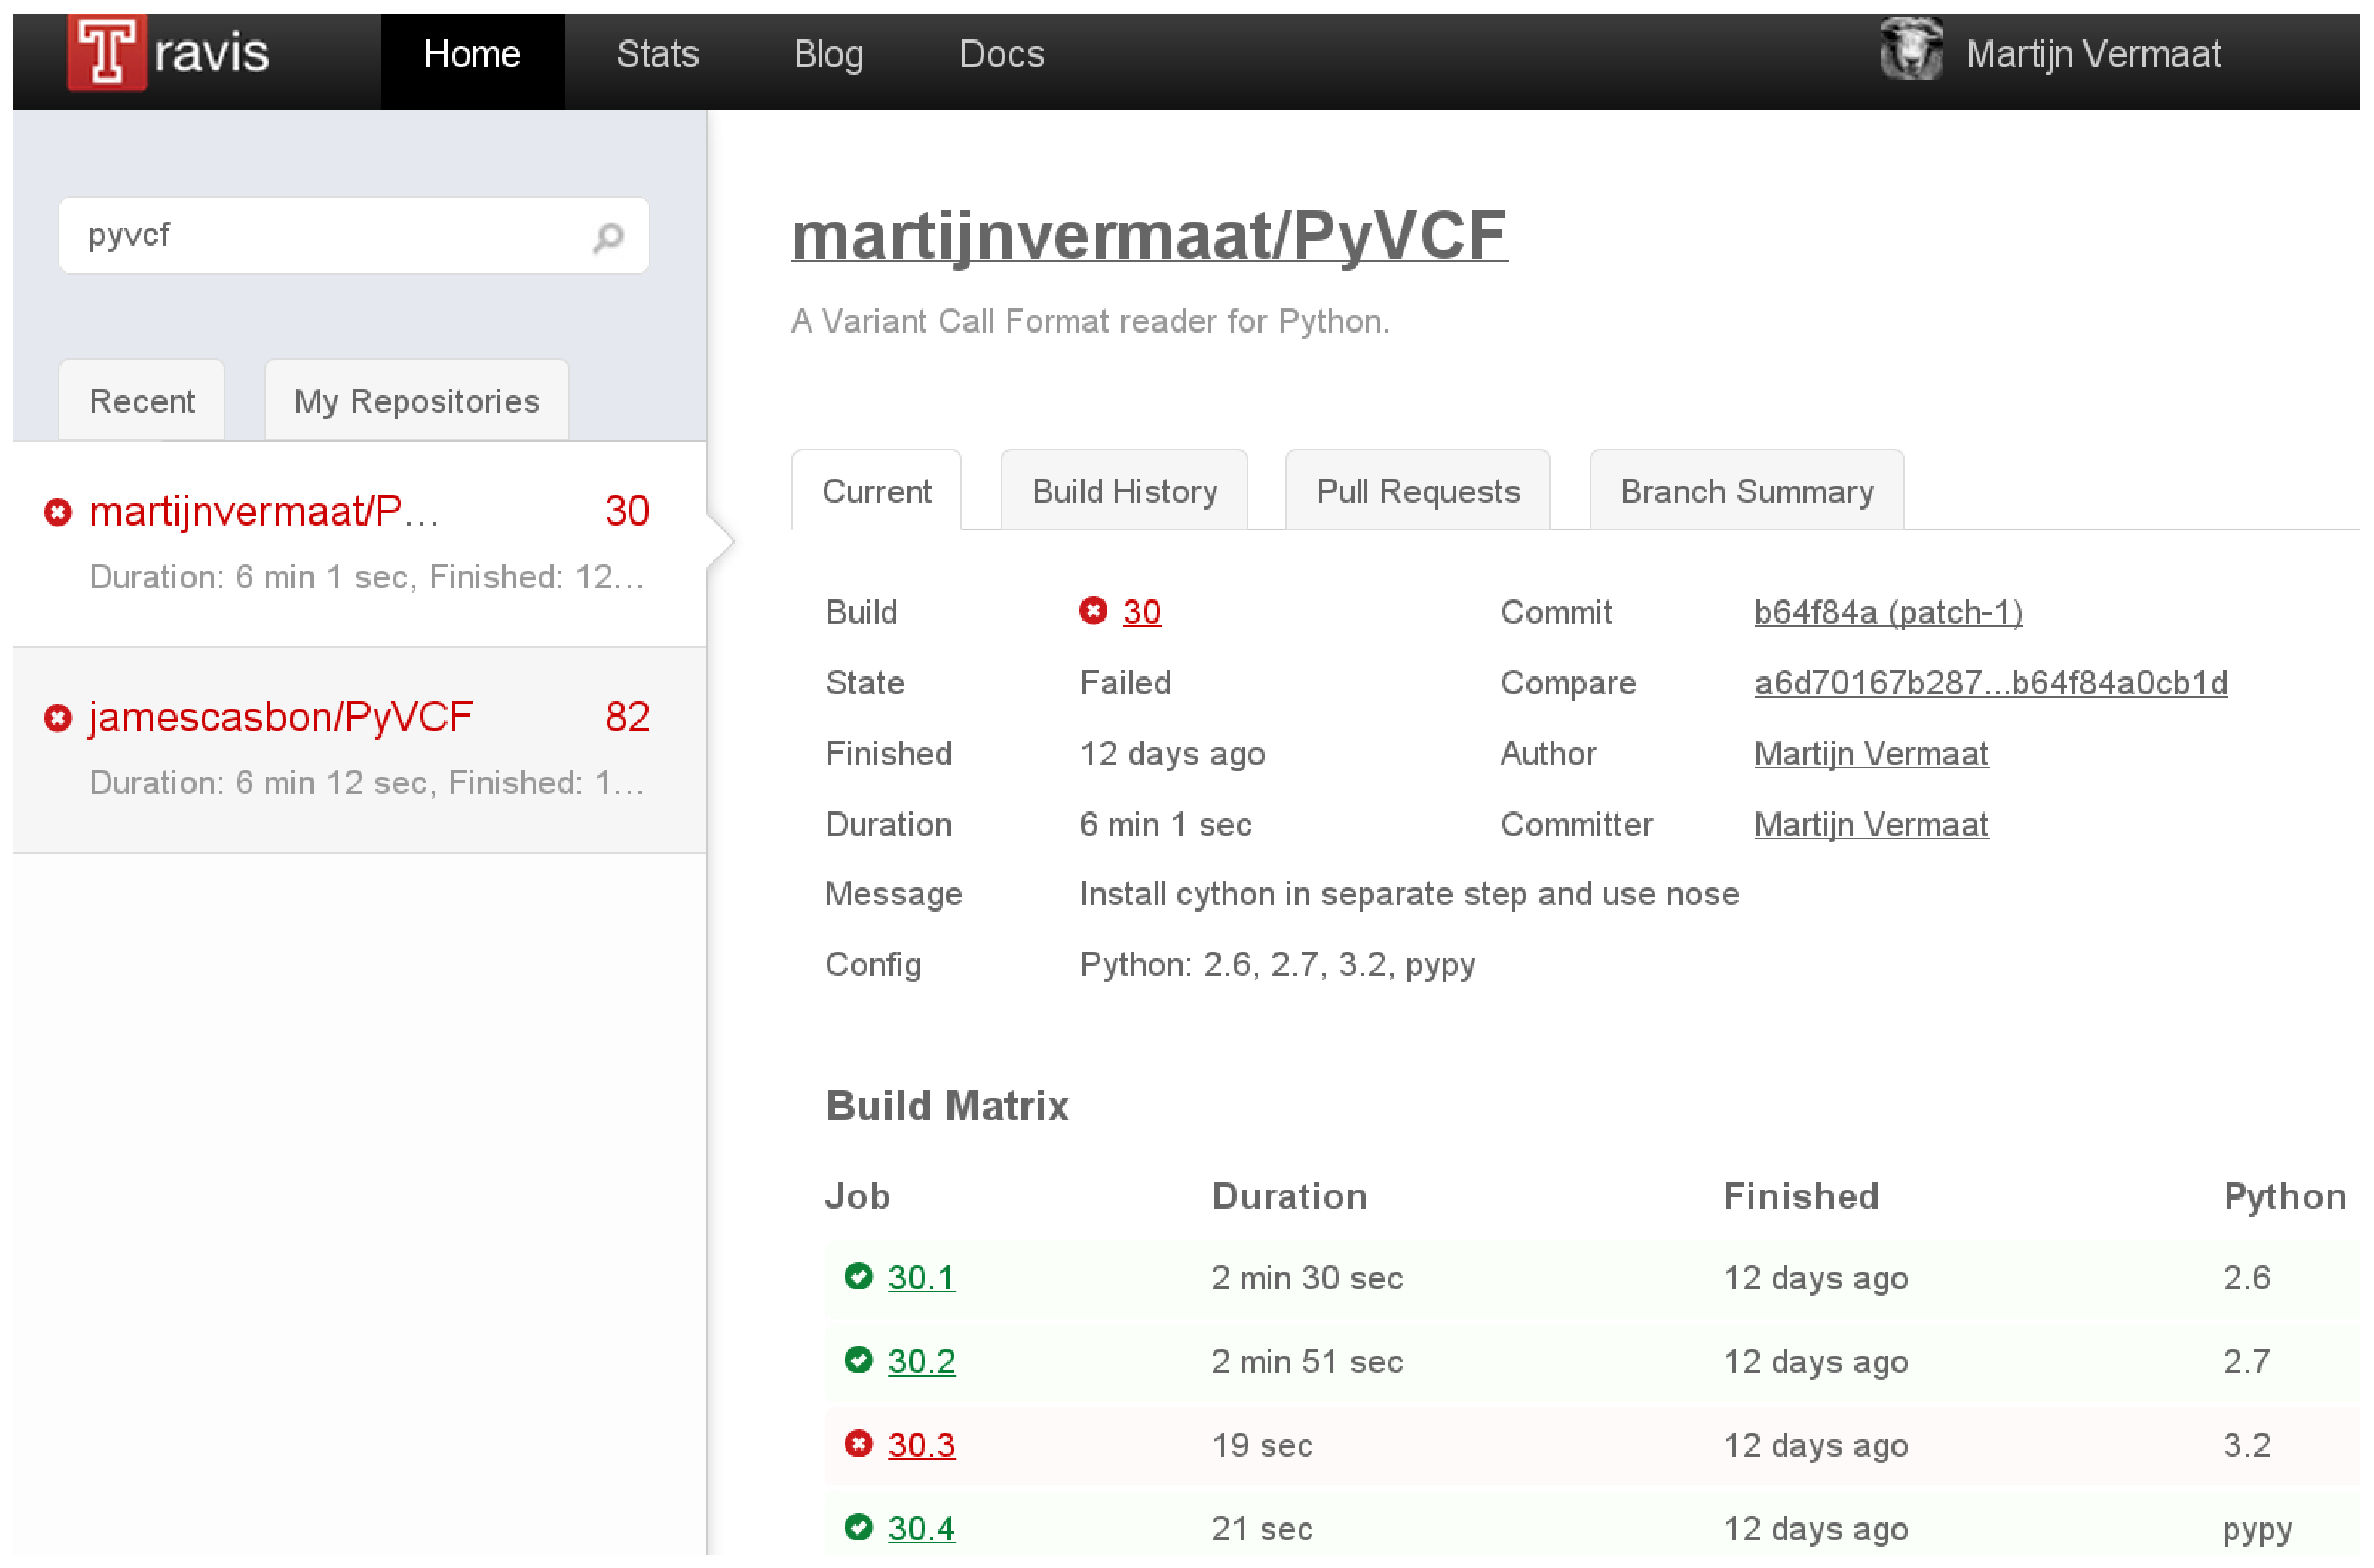
\includegraphics[width=0.9\paperwidth,keepaspectratio=true]{travis}
      \end{center} \vfill}
  }
  \frame{}
}

\begin{frame}
  \frametitle{The ten commandments of scientific coding}
  \begin{enumerate}
    \item Thou shall use version control
    \item Thou shall comment thy code
    \item Thou shall use existing libraries whenever possible
    \item Thou shall try to unit test
    \item Thou shall not make up statistical procedures
    \item {\bf Thou shall read code other than thy own}
    \item Thou shall write documentation
    \item Thou shall beware of floating point issues
    \item Thou shall write modular code
    \item Thou shall follow coding standards
  \end{enumerate}
\end{frame}

\begin{frame}
  \frametitle{Thou shall read code other than thy own}
  \begin{itemize}
    \item Like academics should keep up with the literature
    \item Prevents isolation and tunnel vision
    \item Code review (idealy pre-merge)
  \end{itemize}
\end{frame}

{
  \setbeamercolor{background canvas}{bg=}
  \usebackgroundtemplate{
    \parbox[c][\paperheight]{\paperwidth}{%
      \vfill \begin{center}
      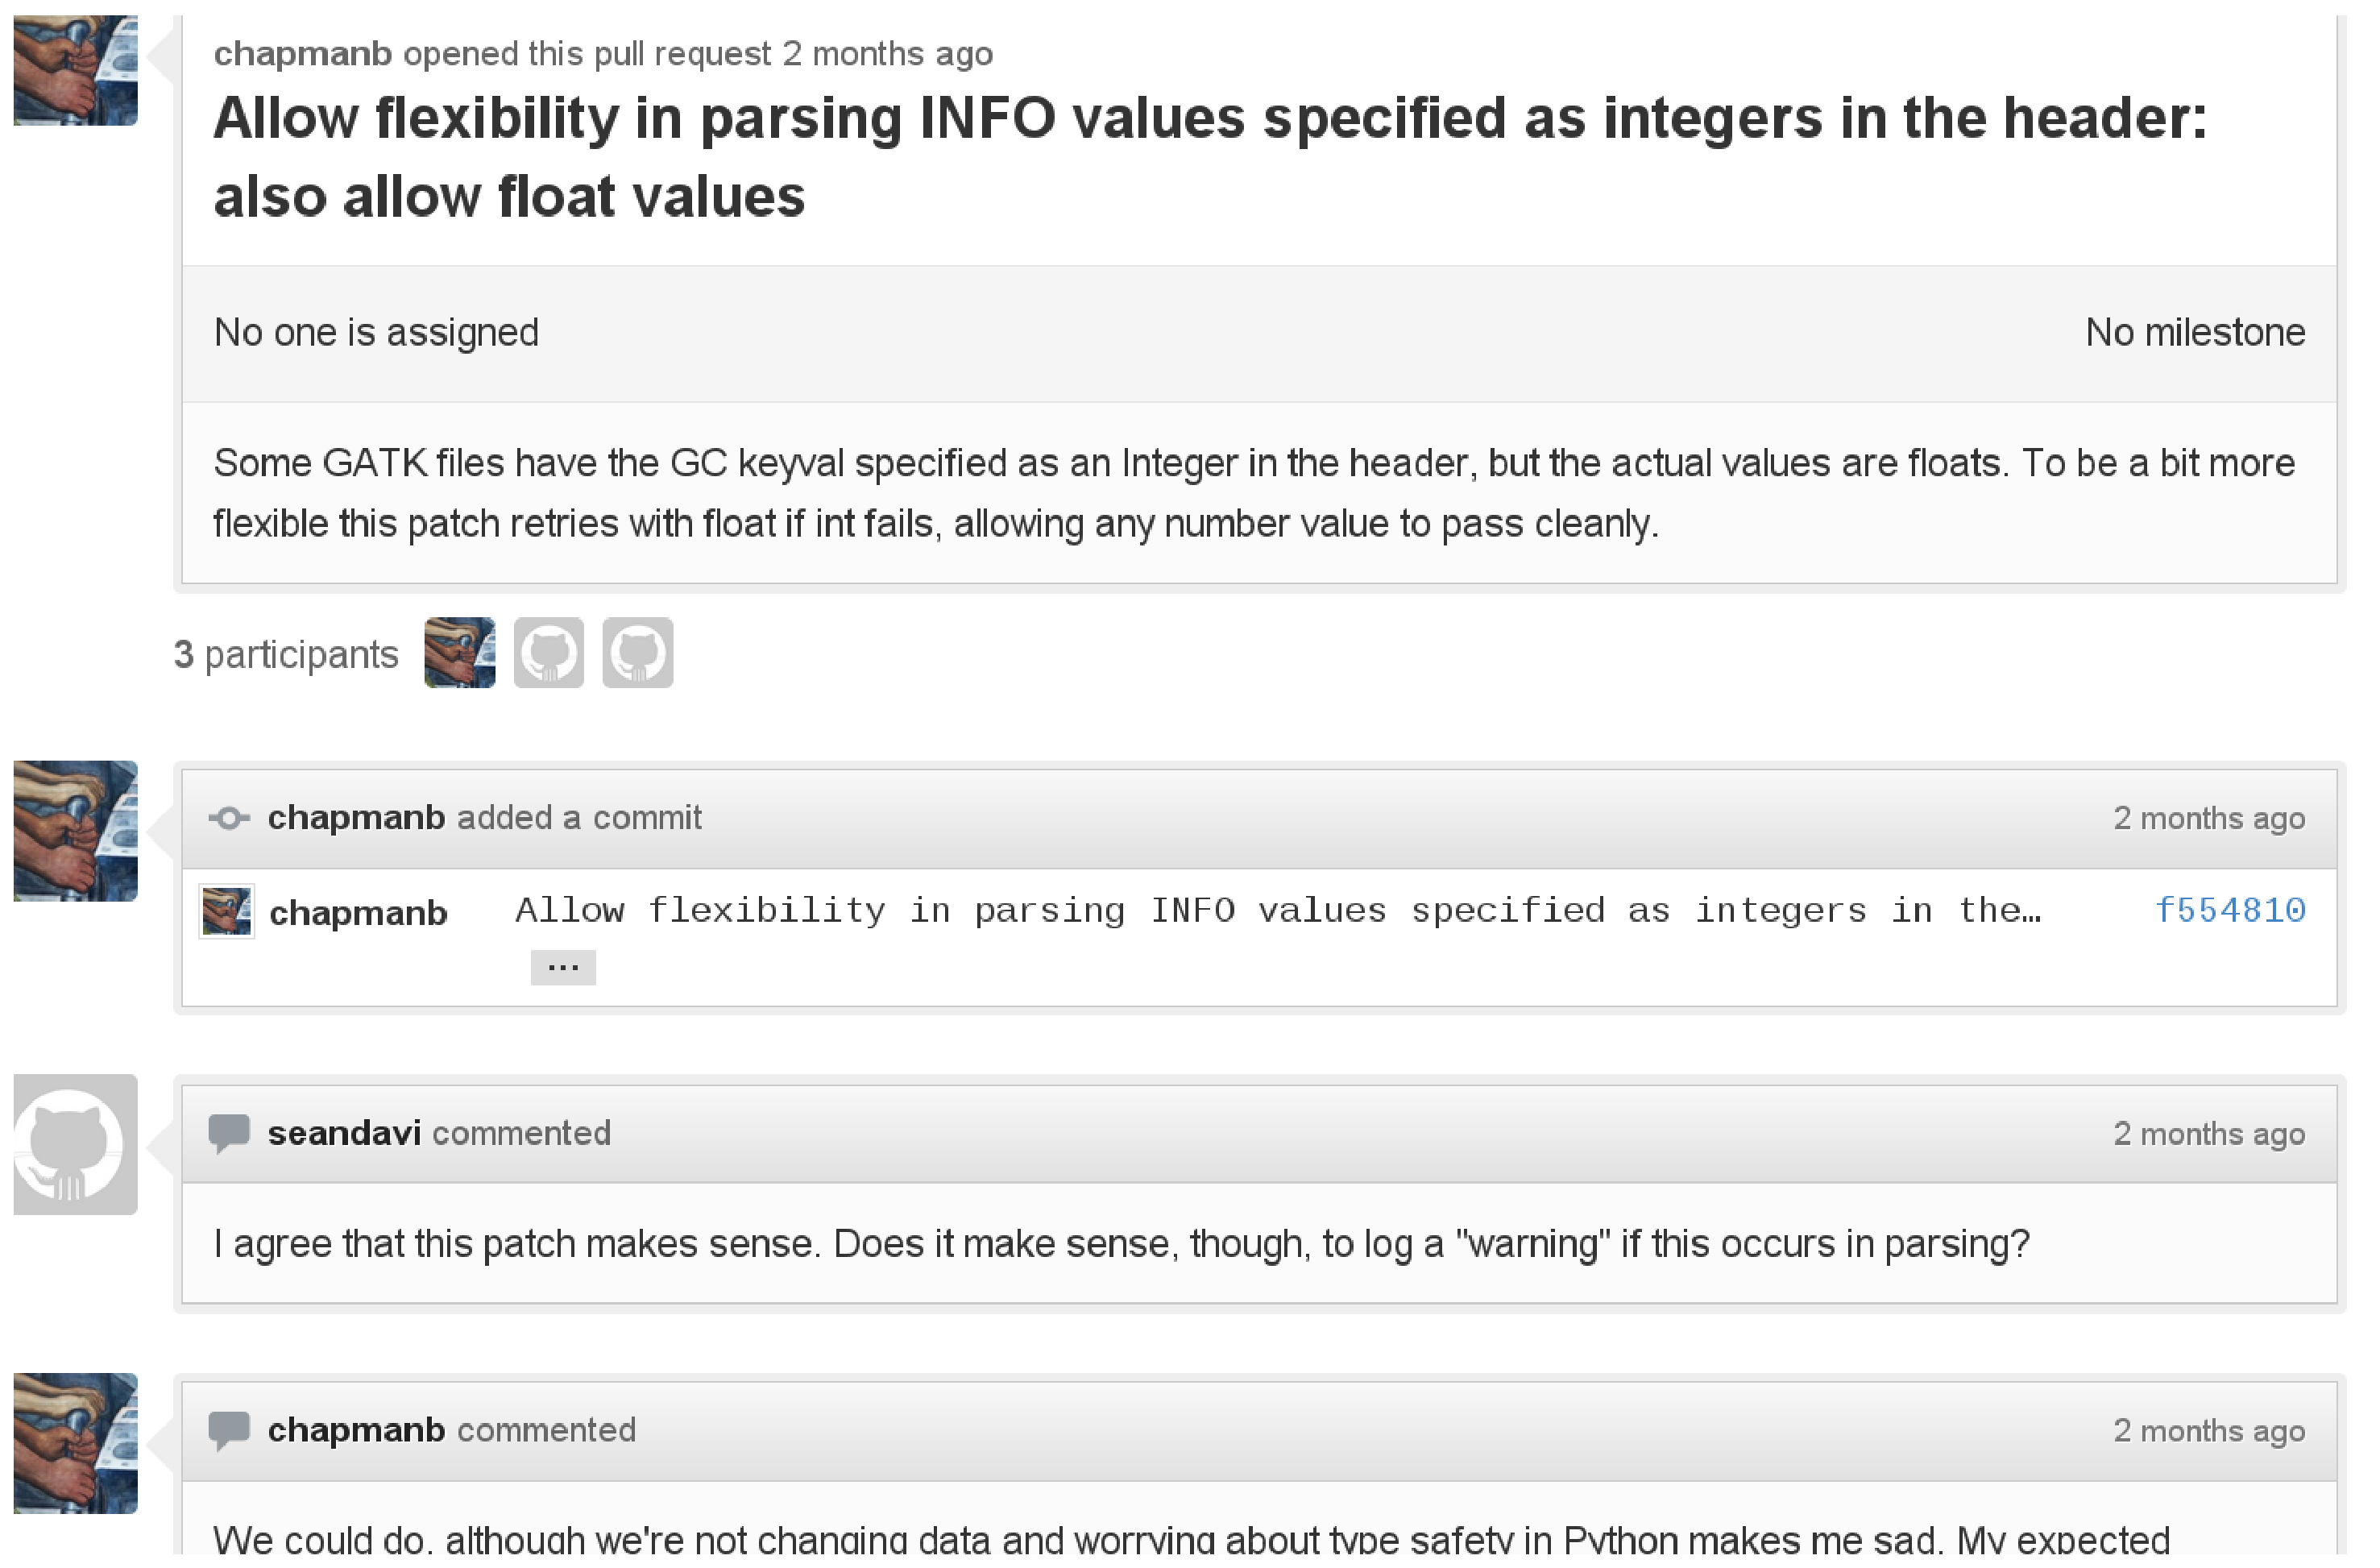
\includegraphics[width=0.9\paperwidth,keepaspectratio=true]{review}
      \end{center} \vfill}
  }
  \frame{}
}

{
  \setbeamercolor{background canvas}{bg=}
  \usebackgroundtemplate{
    \parbox[c][\paperheight]{\paperwidth}{%
      \vfill \begin{center}
      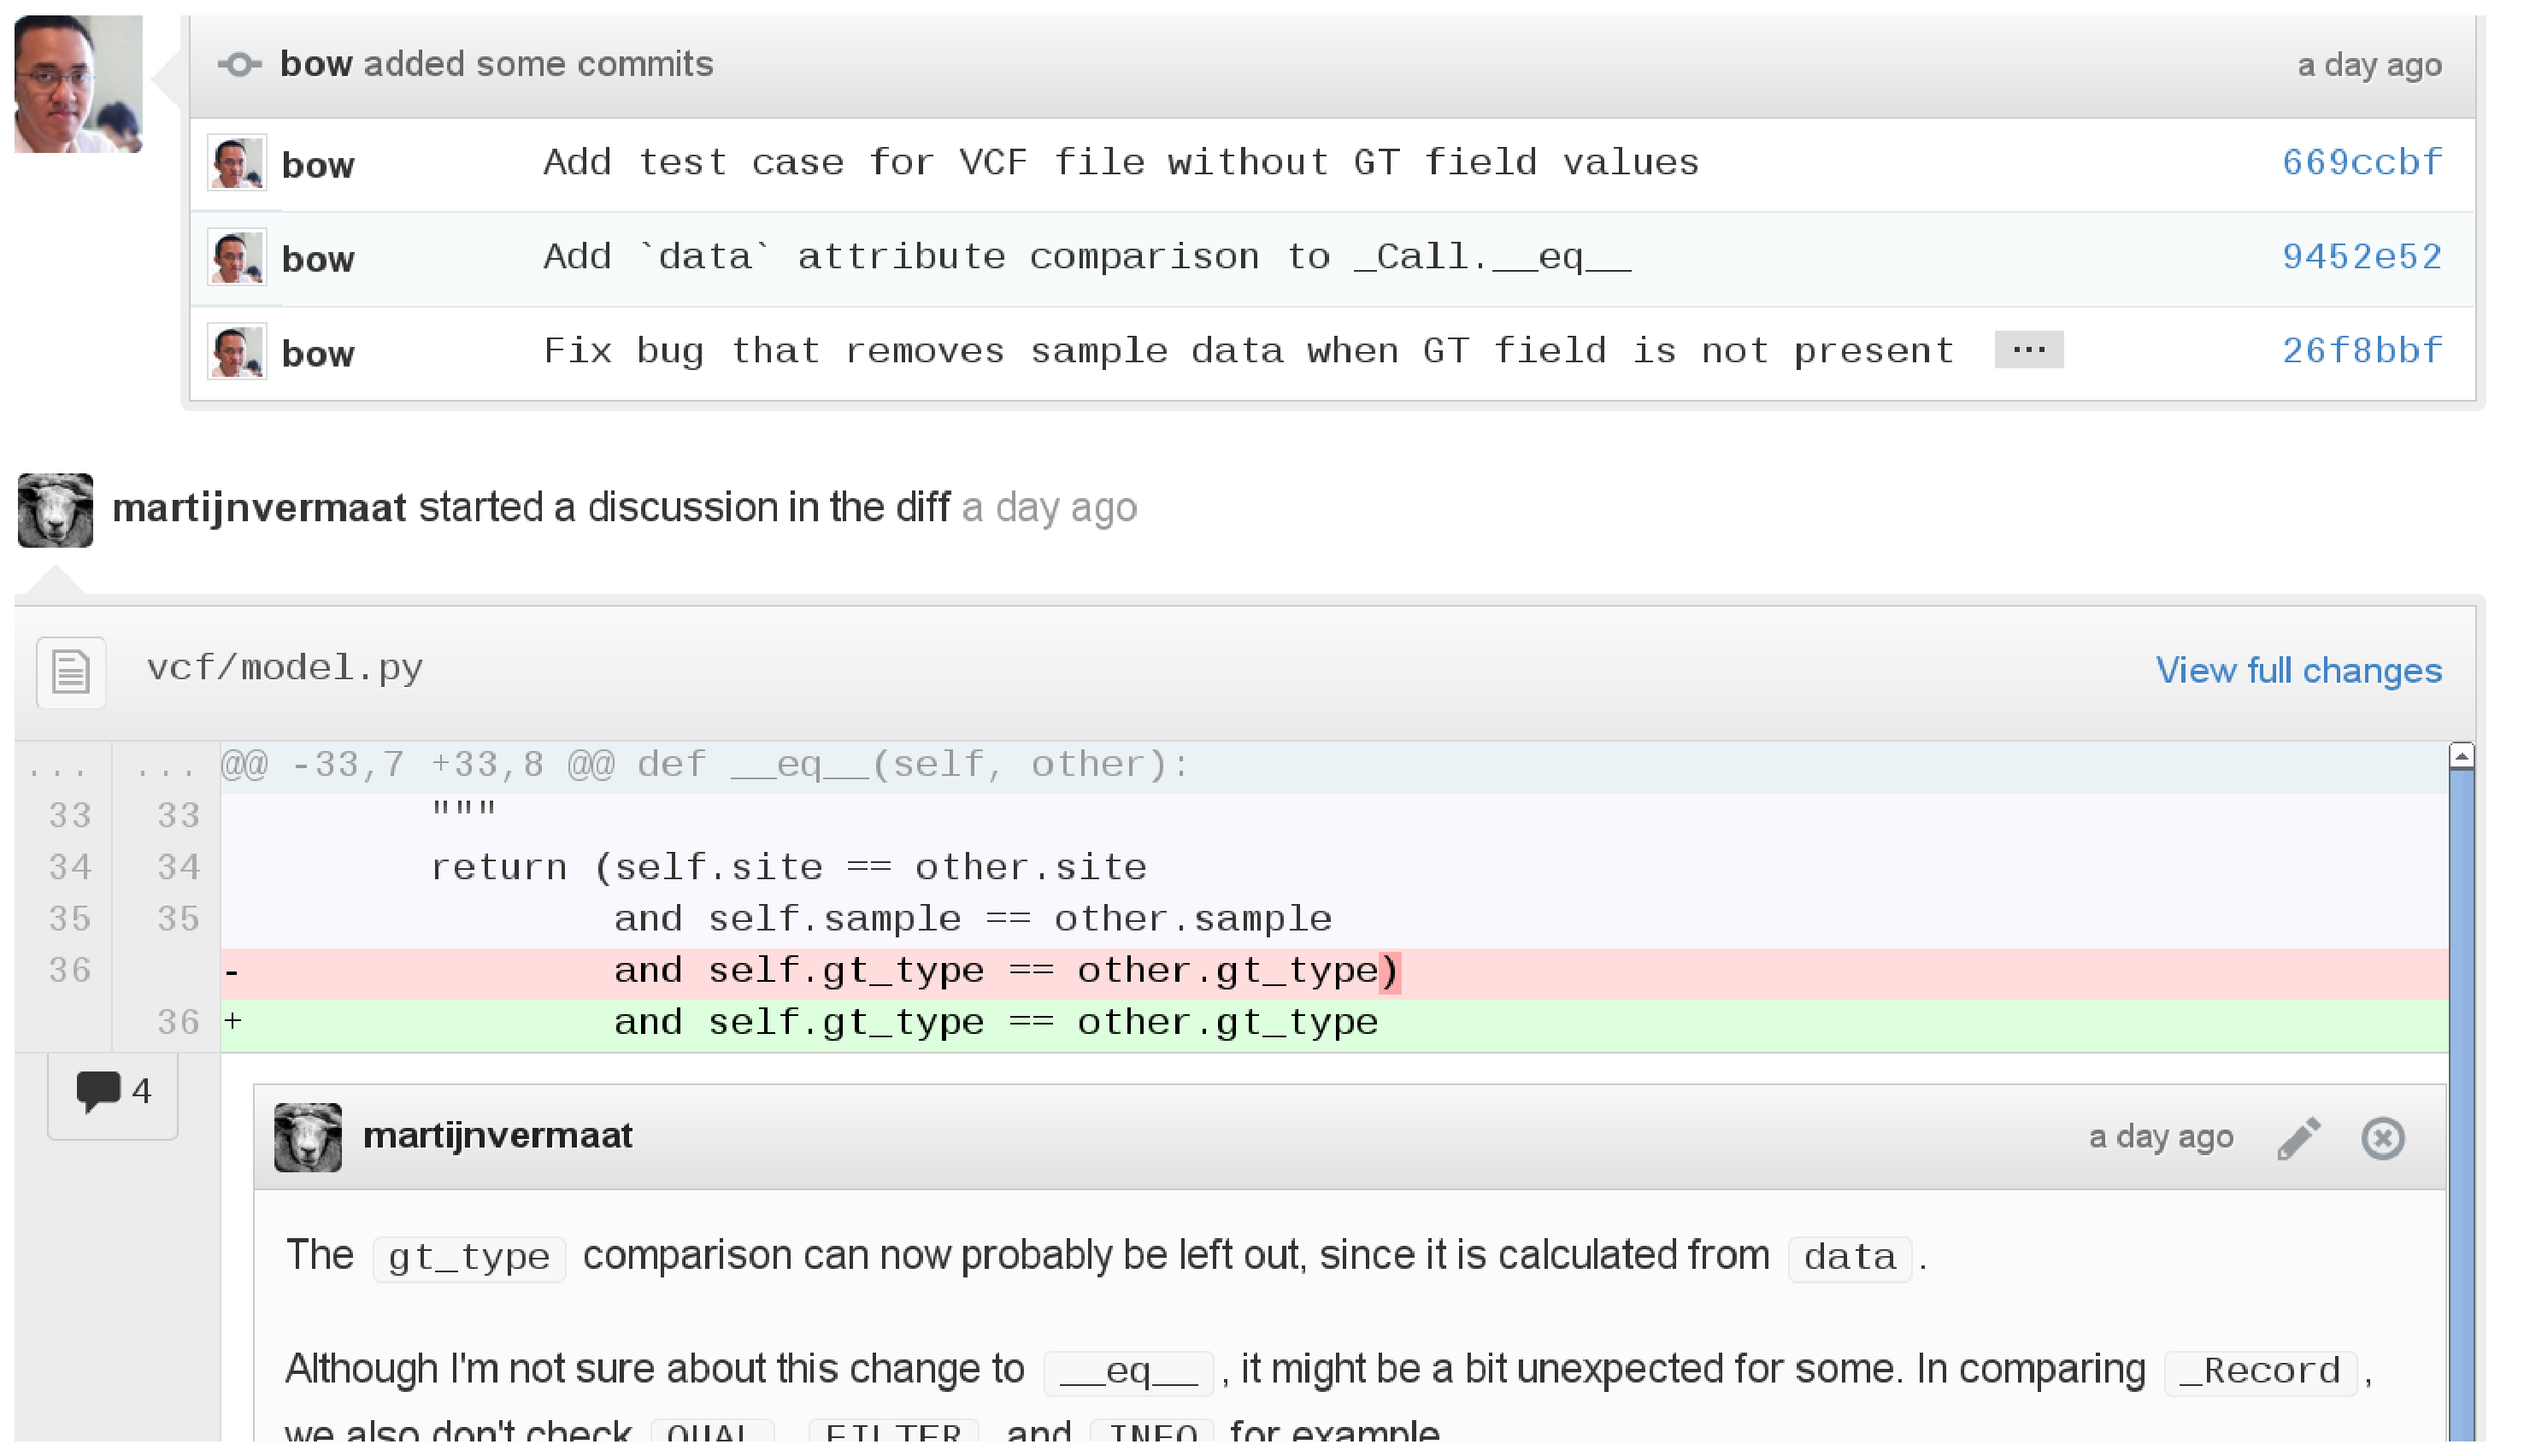
\includegraphics[width=0.9\paperwidth,keepaspectratio=true]{comments}
      \end{center} \vfill}
  }
  \frame{}
}

\begin{frame}
  \frametitle{The ten commandments of scientific coding}
  \begin{enumerate}
    \item Thou shall use version control
    \item Thou shall comment thy code
    \item Thou shall use existing libraries whenever possible
    \item Thou shall try to unit test
    \item Thou shall not make up statistical procedures
    \item Thou shall read code other than thy own
    \item {\bf Thou shall write documentation}
    \item Thou shall beware of floating point issues
    \item Thou shall write modular code
    \item Thou shall follow coding standards
  \end{enumerate}
\end{frame}

{
  \setbeamercolor{background canvas}{bg=}
  \usebackgroundtemplate{
    \parbox[c][\paperheight]{\paperwidth}{%
      \vfill \begin{center}
      
\includegraphics[width=0.9\paperwidth,keepaspectratio=true]{overlyhonestmethods}
      \end{center} \vfill}
  }
  \frame{}
}

\begin{frame}
  \frametitle{Thou shall write documentation}
  \begin{itemize}[<+->]
    \item For users and for developers
    \item Interfaces and reasons, not implementations
    \item Refactor rather than explain
    \item Idealy embedded in the software
  \end{itemize}
\end{frame}

\begin{frame}
  \frametitle{The ten commandments of scientific coding}
  \begin{enumerate}
    \item Thou shall use version control
    \item Thou shall comment thy code
    \item Thou shall use existing libraries whenever possible
    \item Thou shall try to unit test
    \item Thou shall not make up statistical procedures
    \item Thou shall read code other than thy own
    \item Thou shall write documentation
    \item Thou shall beware of floating point issues
    \item {\bf Thou shall write modular code}
    \item Thou shall follow coding standards
  \end{enumerate}
\end{frame}

\begin{frame}
  \frametitle{Thou shall write modular code}
  \begin{itemize}[<+->]
    \item Generalize instead of copy/paste and edit
    \item Have a single representation for every piece of data
    \item One extreme would be Taverna
  \end{itemize}
\end{frame}

\begin{frame}
  \frametitle{The ten commandments of scientific coding}
  \begin{enumerate}
    \item Thou shall use version control
    \item Thou shall comment thy code
    \item Thou shall use existing libraries whenever possible
    \item Thou shall try to unit test
    \item Thou shall not make up statistical procedures
    \item Thou shall read code other than thy own
    \item Thou shall write documentation
    \item Thou shall beware of floating point issues
    \item Thou shall write modular code
    \item Thou shall follow coding standards
  \end{enumerate}
\end{frame}

{
  \setbeamercolor{background canvas}{bg=}
  \usebackgroundtemplate{
    \parbox[c][\paperheight]{\paperwidth}{%
      \vfill \begin{center}
      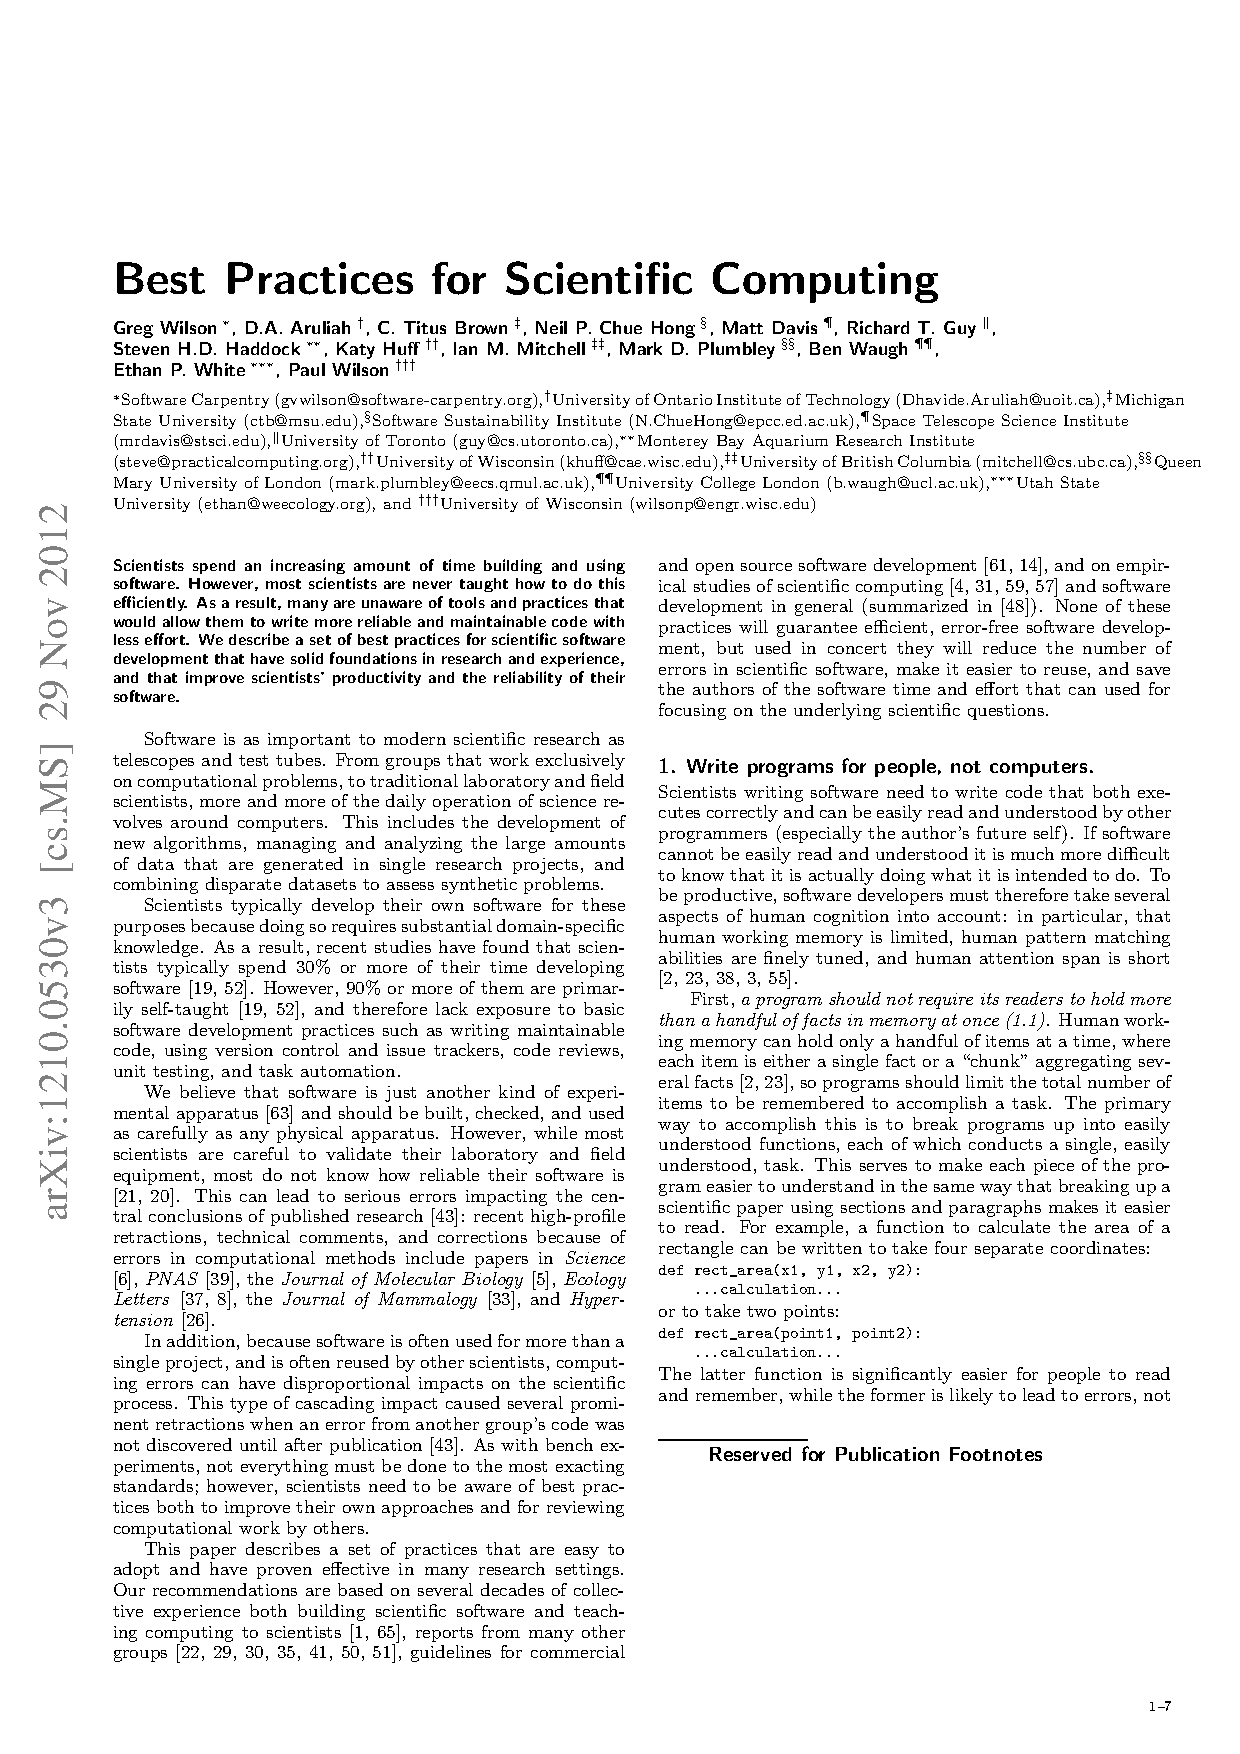
\includegraphics[clip=true,trim=1.5cm 21cm 0cm 0cm,width=\paperwidth,keepaspectratio=true]{practices}
      \end{center}\vspace{3cm} \vfill}
  }
  \frame{}
}

\begin{frame}
  \frametitle{Best practices for scientific computing}
  \begin{enumerate}
    \item Write programs for people, not computers
    \item Automate repetitive tasks
    \item Use the computer to record history
    \item Make incremental changes
    \item Use version control
    \item Don't repeat yourself (or others)
    \item Plan for mistakes
    \item Optimize software only after it works correctly
    \item Document design and purpose, not mechanics
    \item Collaborate
  \end{enumerate}
\end{frame}

\begin{frame}
  \frametitle{Initiatives}
  \begin{itemize}
    \item Science Code Manifesto
    \item Bioinformatics Testing Consortium
    \item Software Carpentry
    \item Our programming course
  \end{itemize}
\end{frame}

{
  \setbeamercolor{background canvas}{bg=}
  \usebackgroundtemplate{
    \parbox[c][\paperheight]{\paperwidth}{%
      \vfill \begin{center}
      
\includegraphics[width=0.8\paperwidth,keepaspectratio=true]{manifesto}
      \end{center} \vfill}
  }
  \frame{}
}

\begin{frame}
  \frametitle{Programming course with Python}
  Why Python?
  \begin{itemize}
    \item Language itself (level of abstraction, syntax)
    \item Suitable for exploratory research
    \item Investement of scientific community and our department
    \item Many bioinformatics tools available
  \end{itemize}
\end{frame}

\section*{Open and Reproducible Scientific Programming}

\begin{frame}
  \frametitle{Conclusions}
  \begin{itemize}
    \item Disclosure and publication requirements for source code is not in
      line with other types of scientific data and materials
    \item This is changing
    \item There is no good reason not to open code
    \item Tool support for managing scientific code
    \item Many best practices are available
  \end{itemize}
\end{frame}

\section*{Questions?}
\lastpagetemplate
\begin{frame}
  \begin{center}
    Acknowledgements:\\
    \vspace{0.8cm}
    Jeroen Laros\\
    Leon Mei\\
    Johan den Dunnen
  \end{center}
  \vspace{1cm}
  {\tiny
    Links to all sources are included on last slide
  }
\end{frame}

\section*{Extra}

\extrapagetemplate
\begin{frame}
  \frametitle{Stop Hosting Data and Code on your Lab Website (1)}
  Survey of URL stability:
  \begin{itemize}
    \item Of 1630 URLs identified in Pubmed abstracts only 63\% were
      consistently available
    \item That rate was far worse for anonymous login FTP sites (33\%)
  \end{itemize}
  Wren, Jonathan D. 404 not found: the stability and persistence of URLs
  published in MEDLINE. Bioinformatics 20.5 (2004): 668-672.
\end{frame}

\extrapagetemplate
\begin{frame}
  \frametitle{Stop Hosting Data and Code on your Lab Website (2)}
  Survey of 1000 web services published in Nucleic Acids Web
  Server Issue (2003--2009):
  \begin{itemize}
    \item 72\% available at the published address
    \item Unable to test functionality for 33\% because of no example data,
      13\% not working as expected
    \item Positive functionality confirmed for 45\%
    \item 274 of 872 corresponding authors answered email
    \item Of these 78\% said a service was developed by a student or temporary
      researcher, and many had no plan for maintenance after the researcher
      had moved on to a permanent position
  \end{itemize}
  Schultheiss, Sebastian J., et al. Persistence and availability of web
  services in computational biology. PLoS one 6.9 (2011): e24914.
\end{frame}

\section*{Sources}
\extrapagetemplate
\begin{frame}
  Clickable links, in no particular order

  \vspace{0.3cm}

  {\fontsize{3.5}{5}\selectfont
    \href{http://www.nature.com/nbt/journal/v28/n11/full/nbt1110-1181.html}{J.T. Dudley and A.J. Butte. In silico research in the era of cloud computing. Nature Biotechnology 28, 1181--1185 (2010)}\\
    \href{http://www.sciencemag.org/content/336/6078/159.summary}{A. Morin et al. Shining Light into Black Boxes. Science 13 April 2012: Vol. 336 no. 6078 pp. 159-160}\\
    \href{http://www.nature.com/nature/journal/v482/n7386/full/nature10836.html}{D.C. Ince, L. Hatton and J. Graham-Cumming. The case for open computer programs. Nature 482, 485--488 (23 February 2012)}\\
    \href{http://www.sciencemag.org/content/331/6018/649.summary}{B. Hanson, A. Sugden, and B. Alberts. Making Data Maximally Available. Science 11 February 2011: Vol. 331 no. 6018 p. 649}\\
    \href{http://www.nature.com/nature/journal/v470/n7334/full/470305b.html}{Editorial. Devil in the details. Nature 470, 305--306 (17 February 2011)}\\
    \href{http://www.sciencemag.org/content/334/6060/1226.abstract}{R.D. Peng. Reproducible Research in Computational Science. Science 2 December 2011: Vol. 334 no. 6060 pp. 1226--1227}\\
    \href{http://online.liebertpub.com/doi/abs/10.1089/omi.2006.10.94}{C. Brooksbank and J. Quackenbush. Data Standards: A Call to Action. OMICS: A Journal of Integrative Biology. June 2006, 10(2): 94--99}\\
    \href{http://arxiv.org/abs/1210.0530}{G. Wilson et al. Best Practices for Scientific Computing. Preprint, arXiv:1210.0530, 29 Nov 2012}\\
    \href{http://arxiv.org/abs/1010.1092}{K.A. Baggerly and K.R. Coombes. Deriving chemosensitivity from cell lines: Forensic bioinformatics and reproducible research in high-throughput biology. Preprint, arXiv:1010.1092, 6 Oct 2010}\\
    \href{http://www.nature.com/news/2010/101013/full/467775a.html}{Z. Merali. Computational science: ...Error. Nature 467, 775--777 (2010)}\\
    \href{https://www.zotero.org/scottbot/items/itemKey/GCQEH25G}{B. D. McCullough et al. Lessons from the JMCB Archive. Journal of Money, Credit, and Banking. Volume 38, Number 4, June 2006}\\
    \href{http://www.ncbi.nlm.nih.gov/pubmed/16646837}{R. Gentleman. Reproducible research: a bioinformatics case study. Stat Appl Genet Mol Biol. 2005;4:Article2. Epub 2005 Jan 11}\\
    \href{http://www.nature.com/news/2010/101013/full/467753a.html}{N. Barnes. Publish your computer code: it is good enough. Nature 467, 753 (2010)}\\
    \href{http://www.oxfordjournals.org/our_journals/bioinformatics/for_authors/general.html}{Oxford Bioinformatics Instructions to Authors}\\
    \href{http://www.plosone.org/static/publication}{PLOS ONE Publication Criteria}\\
    \href{http://www.galter.northwestern.edu/news/index.cfm/2012/10/9/Datasets-Software-Eligible-for-Listing-in-NSF-Biosketches}{P. Shaw. Datasets, Software Eligible for Listing in NSF Biosketches. Galter Health Sciences Library website (9 October 2012}\\
    \href{http://scofield.bx.psu.edu/~dannon/encodevm/}{ENCODE Virtual Machine and Cloud Resource}\\
    \href{http://simplystatistics.org/2013/01/23/statisticians-and-computer-scientists-if-there-is-no-code-there-is-no-paper/}{J. Leek. Statisticians and computer scientists -- if there is no code, there is no paper. Simply Statistics (23 January 2013)}\\
    \href{http://www.bendmorris.com/2012/12/what-incentives-are-there-to-maintain.html}{B. Morris. What incentives are there to maintain software in academia? Ben Morris' Macroblog (29 December, 2012)}\\
    \href{http://gettinggeneticsdone.blogspot.nl/2013/01/stop-hosting-data-and-code-on-your-lab.html}{S. Turner. Stop Hosting Data and Code on your Lab Website. Getting Genetics Done (8 January 2013))}\\
    \href{http://www.johndcook.com/blog/2010/10/19/buggy-simulation-code-is-biased/}{J.D. Cook. Buggy code is biased code. The Endeavour (19 October 2010)}\\
    \href{https://gist.github.com/3311557}{V. Buffalo. The Ten Commandments of Scientific Coding. GitHub Gist (8 Oct 2012)}\\
    \href{http://www.slideshare.net/jandot/b-temperton-the-bioinformatics-testing-consortium}{B. Temperton. The Bioinformatics Testing Consortium. BOSC2012 (Jul 16, 2012)}\\
    \href{https://speakerdeck.com/ptomato/open-and-reproducible-scientific-programming}{P. Chimento. Open and reproducible scientific programming. Apr 5, 2012}\\
    \href{http://www.osnews.com/story/19266/WTFs_m}{OSNews on WTFs/m}\\
    \href{https://twitter.com/ianholmes/status/288689712636493824}{Ian Holmes (@ianholmes) on Twitter about \#overlyhonestmethods}\\
    \href{https://twitter.com/luispedrocoelho/status/238632048313647104}{Luis Pedro Coelho (@luispedrocoelho) on Twitter about scientists ashamed of their code}\\
    \href{https://twitter.com/ianholmes/status/250608615361241089}{Ian Holmes (@ianholmes) on Twitter about biologists, physicists and preprints (1)}\\
    \href{https://twitter.com/ianholmes/status/250608825428746242}{Ian Holmes (@ianholmes) on Twitter about biologists, physicists and preprints (2)}\\
    \href{http://jrjohansson.github.com/}{R. Johansson. Lectures on scientific computing with Python}\\
    \href{http://matt.might.net/articles/crapl/}{M. Might. The CRAPL: An academic-strength open source license}\\
    \href{http://sciencecodemanifesto.org/}{Science Code Manifesto}\\
    \href{http://biotest.cgrb.oregonstate.edu/}{Bioinformatics Testing Consortium}\\
    \href{http://software-carpentry.org/}{Software Carpentry}\\
    \href{http://ipython.org/}{F. P\'erez and B.E. Granger. IPython: a System for Interactive Scientific Computing. Science and Engineering, vol. 9, no. 3, pp. 21--29, May/June 2007}\\
    \href{https://travis-ci.org/}{Travis CI. A hosted continuous integration service for the open source community}\\
    \href{https://github.com/}{GitHub. Build software better, together}\\
  }
\end{frame}

\end{document}
